% Created 2020-08-19 Wed 07:58
% Intended LaTeX compiler: pdflatex
\documentclass[11pt]{article}
\usepackage[utf8]{inputenc}
\usepackage[T1]{fontenc}
\usepackage{graphicx}
\usepackage{grffile}
\usepackage{longtable}
\usepackage{wrapfig}
\usepackage{rotating}
\usepackage[normalem]{ulem}
\usepackage{amsmath}
\usepackage{textcomp}
\usepackage{amssymb}
\usepackage{capt-of}
\usepackage{hyperref}
\usepackage{minted}
\IfFileExists{./resources/lllstyle}{\usepackage{resources/style}}{}
\IfFileExists{./resources/referencing.sty}{\usepackage{resources/referencing}}{}
\addbibresource{resources/references.bib}
\author{Ryan Greenup}
\date{\today}
\title{Data Sci Discover Project}
\hypersetup{
 pdfauthor={Ryan Greenup},
 pdftitle={Data Sci Discover Project},
 pdfkeywords={},
 pdfsubject={},
 pdfcreator={Emacs 26.3 (Org mode 9.4)}, 
 pdflang={English}}
\begin{document}

\maketitle
\tableofcontents


\section{Links}
\label{sec:orgd8cac5a}
\begin{itemize}
\item \href{Proposal/Propsal.org}{Research Proposal}
\item \href{laparkPowerWalk2013.pdf}{Paper}
\item \href{ImplementingPageRank/01PageRank.Rmd}{Preliminary Implementation}
\item \href{ImplementingPageRank/01PageRank.R}{Implement Random Surfer on Sparse Matrix}
\item \href{ImplementingPowerWalk/01PowerWalk.R}{Implement Power Walk on Sparse Matrix}
\end{itemize}



\section{Proposal}
\label{sec:org611f515}

\subsection{Question}
\label{sec:org1f2d35c}

\emph{Can we determine the second eigenvalue from the method parameters? For PageRank, the second eigenvalue is equal to the smoothing parameter \(\alpha\)}

\begin{quote}
Yes. An open question for the Power Walk method is, can we determine the second eigenvalue from the method parameters? For PageRank, the second eigenvalue is equal to the smoothing parameter \(\alpha\). The second eigenvalue determines how long the algorithm takes to converge and how stable the solution is.
To begin, implement the method for computing PageRank and then the Power Walk. It can all be done using sparse matrices, so it only requires a fraction of the memory and is each iteration is quick.
\end{quote}

\subsection{Working}
\label{sec:orgedb3342}

Take the exemplar Graph from Figure 1:


\begin{center}
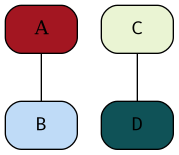
\includegraphics[width=.9\linewidth]{./Media/Example.png}
\end{center}



\begin{align}
    \Gamma =  I - n D^{- 1}_B \\
\end{align}

Where we have the following:

\begin{align}
    \beta &= 10 \\
    B &= \beta^A \\
    A &=
    \begin{bmatrix}
0& 1& 0& 0 \\
1& 0& 0& 0 \\
0& 0& 0& 1 \\
0& 0& 1& 0
    \end{bmatrix} \\
     \implies
    B &= \begin{bmatrix}
     10 & 1 & 1 & 1 \\
     1 & 10 & 1 & 1 \\
     1 & 1 & 10 & 1 \\
     1 & 1 & 1 & 10 \\
     \end{bmatrix}  \\
     \text{$D_B$ is a diagonal matrix of the column sums:}\\
     D &= \begin{bmatrix}
     13 & 0 & 0 & 0 \\
     0 & 13 & 0 & 0 \\
     0 & 0 & 13 & 0 \\
     0 & 0 & 0 & 13
     \end{bmatrix}  \\
     \text{Hence the Inverse is:}\\
     D_B^{-1}&= \frac{I}{13}\\
     \text{Putting it all together:}\\
     \Gamma &=  I - n D^{- 1}_B \\
     &= I - \frac{4 \cdot I}{13} \\
     &= \frac{9}{13} \cdot  I \\
     &= \begin{bmatrix}
         \frac{9}{13} & 0 & 0 & 0 \\
         0 & \frac{9}{13} & 0 & 0 \\
         0 & 0 & \frac{9}{13} & 0 \\
         0 & 0 & 0 &  \frac{9}{13}
     \end{bmatrix}  \\
     & \approx \begin{bmatrix}
         0.6923 & 0 & 0 & 0 \\
         0 & 0.6923 & 0 & 0 \\
         0 & 0 & 0.6923 & 0 \\
         0 & 0 & 0 & 0.6923
     \end{bmatrix}
\end{align}




\section{Working}
\label{sec:org53d06b1}
\begin{minted}[]{r}
  if (require("pacman")) {
      library(pacman)
    }else{
      install.packages("pacman")
      library(pacman)
    }
\end{minted}
\begin{minted}[]{r}
    pacman::p_load(tidyverse, Matrix, igraph, plotly, mise, docstring)
\end{minted}

\subsection{Implementing Page Rank Method on a small graph}
\label{sec:orgd1c7271}
\subsubsection{Example Graph}
\label{sec:orgb098a3f}
Consider the following Graph taken from the paper:

\begin{minted}[]{r}
  g1 <- igraph::graph.formula(1++2, 1+-8, 1+-5, 2+-5, 2+-7, 2+-8, 2+-6, 2+-9, 3++4, 3+-5, 3+-6, 3+-9, 3+-10, 4+-9, 4+-10, 4+-5, 5+-8, 6+-8, 7+-8)
  plot(g1)
\end{minted}

\begin{center}
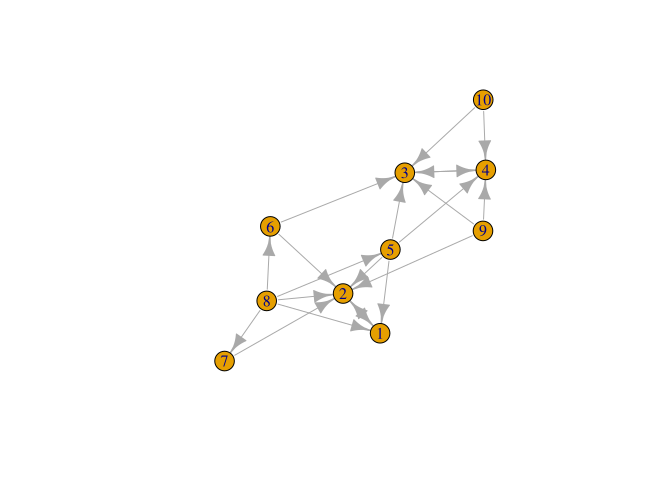
\includegraphics[width=.9\linewidth]{ImplementingPageRank/01PageRank_files/figure-html/unnamed-chunk-2-1.png}
\end{center}

\begin{enumerate}
\item Adjacency Matrix
\label{sec:org39edb0e}
The adjacency Matrix is given by:

\begin{minted}[]{r}
  A <- igraph::get.adjacency(g1, names = TRUE, sparse = FALSE) %>%
    as.matrix()

  ## Adjust the Order
  (A <- A[order(as.integer(row.names(A))), order(as.integer(colnames(A)))])
\end{minted}

\begin{verbatim}
  ##    1 2 3 4 5 6 7 8 9 10
  ## 1  0 1 0 0 0 0 0 0 0  0
  ## 2  1 0 0 0 0 0 0 0 0  0
  ## 3  0 0 0 1 0 0 0 0 0  0
  ## 4  0 0 1 0 0 0 0 0 0  0
  ## 5  1 1 1 1 0 0 0 0 0  0
  ## 6  0 1 1 0 0 0 0 0 0  0
  ## 7  0 1 0 0 0 0 0 0 0  0
  ## 8  1 1 0 0 1 1 1 0 0  0
  ## 9  0 1 1 1 0 0 0 0 0  0
  ## 10 0 0 1 1 0 0 0 0 0  0
\end{verbatim}

\item State Distribution
\label{sec:org66db707}
The state distribution is the transpose of the adjacency matrix:

\begin{minted}[]{r}
  (p0 <- t(A))
\end{minted}

\begin{verbatim}
  ##    1 2 3 4 5 6 7 8 9 10
  ## 1  0 1 0 0 1 0 0 1 0  0
  ## 2  1 0 0 0 1 1 1 1 1  0
  ## 3  0 0 0 1 1 1 0 0 1  1
  ## 4  0 0 1 0 1 0 0 0 1  1
  ## 5  0 0 0 0 0 0 0 1 0  0
  ## 6  0 0 0 0 0 0 0 1 0  0
  ## 7  0 0 0 0 0 0 0 1 0  0
  ## 8  0 0 0 0 0 0 0 0 0  0
  ## 9  0 0 0 0 0 0 0 0 0  0
  ## 10 0 0 0 0 0 0 0 0 0  0
\end{verbatim}

\item Probability Transition Matrix
\label{sec:org035b5f7}
The probability transition matrix is such that each column of the
initial state distribution (i.e. the transposed adjacency matrix) is
scaled to 1.

\begin{minted}[]{r}
  p0 %*% diag(1/colSums(p0))
\end{minted}

\begin{verbatim}
  ##    [,1] [,2] [,3] [,4] [,5] [,6] [,7] [,8]      [,9] [,10]
  ## 1     0    1    0    0 0.25  0.0    0  0.2 0.0000000   0.0
  ## 2     1    0    0    0 0.25  0.5    1  0.2 0.3333333   0.0
  ## 3     0    0    0    1 0.25  0.5    0  0.0 0.3333333   0.5
  ## 4     0    0    1    0 0.25  0.0    0  0.0 0.3333333   0.5
  ## 5     0    0    0    0 0.00  0.0    0  0.2 0.0000000   0.0
  ## 6     0    0    0    0 0.00  0.0    0  0.2 0.0000000   0.0
  ## 7     0    0    0    0 0.00  0.0    0  0.2 0.0000000   0.0
  ## 8     0    0    0    0 0.00  0.0    0  0.0 0.0000000   0.0
  ## 9     0    0    0    0 0.00  0.0    0  0.0 0.0000000   0.0
  ## 10    0    0    0    0 0.00  0.0    0  0.0 0.0000000   0.0
\end{verbatim}

\begin{enumerate}
\item Create a Function
\label{sec:orgc57a2a2}
\begin{minted}[]{r}
  adj_to_probTrans <- function(adjMat) {
    t(adjMat) %*% diag(1/colSums(t(adjMat)))
  }

  (T <- adj_to_probTrans(A)) %>% round(2)
\end{minted}

\begin{verbatim}
  ##    [,1] [,2] [,3] [,4] [,5] [,6] [,7] [,8] [,9] [,10]
  ## 1     0    1    0    0 0.25  0.0    0  0.2 0.00   0.0
  ## 2     1    0    0    0 0.25  0.5    1  0.2 0.33   0.0
  ## 3     0    0    0    1 0.25  0.5    0  0.0 0.33   0.5
  ## 4     0    0    1    0 0.25  0.0    0  0.0 0.33   0.5
  ## 5     0    0    0    0 0.00  0.0    0  0.2 0.00   0.0
  ## 6     0    0    0    0 0.00  0.0    0  0.2 0.00   0.0
  ## 7     0    0    0    0 0.00  0.0    0  0.2 0.00   0.0
  ## 8     0    0    0    0 0.00  0.0    0  0.0 0.00   0.0
  ## 9     0    0    0    0 0.00  0.0    0  0.0 0.00   0.0
  ## 10    0    0    0    0 0.00  0.0    0  0.0 0.00   0.0
\end{verbatim}
\end{enumerate}
\end{enumerate}

\subsubsection{Page Rank Random Surfer}
\label{sec:org9cdc1f7}
The random surfer page rank method modifies the probability transition
matrix \(T\) so that the method works also for non-ergodic graphs by
introducing the possibility of a random jump, we'll call the surfer
transition matrix \(S\):

\begin{align}
    S &= \lambda T +  \left( 1- \lambda \right)B :\\
\ \\
    B&= \begin{bmatrix}
    \frac{1}{N} & \frac{1}{N} & \ldots & \frac{1}{N} \\
    \frac{1}{N} & \frac{1}{N} & \ldots & \frac{1}{N} \\
        \vdots      & \vdots      & \ddots & \vdots \\
    \frac{1}{N} & \frac{1}{N} & \ldots & \frac{1}{N} \\
    \end{bmatrix}  \\
    N&= \left| \left| V \right| \right| \\
    \lambda &\in [0,1]
\end{align}

\begin{minted}[]{r}
  B <- matrix(rep(1/nrow(T), length.out = nrow(T)**2), nrow = nrow(T))
  l <- 0.8123456789

  S <- l*T+(1-l)*B
\end{minted}

\begin{enumerate}
\item Eigen Value Method
\label{sec:orgebc9380}
The eigenvector corresponding to the the eigenvalue of 1 will be the
stationary point:

\begin{minted}[]{r}
  eigen(S, symmetric = FALSE)
\end{minted}

\begin{verbatim}
eigen() decomposition
$values
 [1]  1.000000e+00 -8.123457e-01 -8.123457e-01  8.123457e-01 -3.407464e-09  3.407464e-09
 [7]  6.878591e-17 -4.393838e-17 -1.126771e-18 -1.292735e-32

$vectors
            [,1]          [,2]          [,3]          [,4]          [,5]          [,6]
 [1,] 0.48726141 -7.071005e-01  1.590774e-03  5.000000e-01  6.735753e-01 -6.735753e-01
 [2,] 0.52676629  7.071005e-01 -1.590774e-03  5.000000e-01  9.622504e-02 -9.622505e-02
 [3,] 0.49149620 -2.975837e-03  7.071050e-01 -5.000000e-01  9.622504e-02 -9.622505e-02
 [4,] 0.48044122  2.975837e-03 -7.071050e-01 -5.000000e-01  2.886751e-01 -2.886751e-01
 [5,] 0.04932738  1.463673e-18 -5.541166e-17  2.124631e-17 -3.849002e-01  3.849002e-01
 [6,] 0.04932738  1.463673e-18  5.541166e-17  2.124631e-17 -3.849002e-01  3.849002e-01
 [7,] 0.04932738  1.463673e-18 -2.077937e-17  2.124631e-17 -3.849002e-01  3.849002e-01
 [8,] 0.04243328 -6.484884e-18 -1.103904e-17  6.319692e-17  8.072508e-09  8.072508e-09
 [9,] 0.04243328  6.952446e-18 -9.740331e-18  6.005334e-17  8.072508e-09  8.072509e-09
[10,] 0.04243328  6.952446e-18 -9.740331e-18  6.005334e-17  8.072508e-09  8.072509e-09
               [,7]          [,8]          [,9]         [,10]
 [1,] -3.963430e-01  3.962600e-01  1.828019e-01 -1.752367e-01
 [2,] -1.291621e-01  2.027302e-01  2.199538e-01 -2.197680e-01
 [3,] -3.955284e-01  3.894308e-02  2.223048e-01 -2.248876e-01
 [4,] -4.215353e-01  1.043870e-01  2.747562e-01 -2.777266e-01
 [5,]  5.166485e-01 -8.109210e-01 -8.798152e-01  8.790721e-01
 [6,]  5.201366e-02 -1.308878e-01 -1.049028e-01  1.056778e-01
 [7,]  1.346275e-01 -1.936007e-01  9.054366e-02 -9.554811e-02
 [8,]  2.547528e-16 -1.352936e-16 -1.025353e-16  1.072771e-16
 [9,]  3.196396e-01  1.965446e-01 -2.821213e-03 -5.466313e-03
[10,]  3.196396e-01  1.965446e-01 -2.821213e-03  1.388344e-02

\end{verbatim}

So in this case \sout{the} a stationary point is
\(\langle -0.49, -0.53, -0.49, -0.48, -0.05, -0.05, -0.05, -0.04, -0.04, -0.04 \rangle\)

which can be verified:

$$
1 \vec{p} = S\vec{p}
$$

\begin{minted}[]{r}
  (p     <- eigen(S)$values[1] * eigen(S)$vectors[,1])
\end{minted}

\begin{verbatim}
  ##  [1] -0.48531271 -0.52732002 -0.49152601 -0.47977477 -0.05288058 -0.05288058
  ##  [7] -0.05288058 -0.04558671 -0.04558671 -0.04558671
\end{verbatim}

\begin{minted}[]{r}
  (p_new <- S %*% p)
\end{minted}

\begin{verbatim}
  ##           [,1]
  ## 1  -0.48531271
  ## 2  -0.52732002
  ## 3  -0.49152601
  ## 4  -0.47977477
  ## 5  -0.05288058
  ## 6  -0.05288058
  ## 7  -0.05288058
  ## 8  -0.04558671
  ## 9  -0.04558671
  ## 10 -0.04558671
\end{verbatim}

However this vector does not sum to 1 so the scale should be adjusted
(for probabilities the vector should sum to 1):

\begin{minted}[]{r}
  (p_new <- p_new/sum(p_new))
\end{minted}

\begin{verbatim}
  ##         [,1]
  ## 1  0.2129185
  ## 2  0.2313481
  ## 3  0.2156444
  ## 4  0.2104889
  ## 5  0.0232000
  ## 6  0.0232000
  ## 7  0.0232000
  ## 8  0.0200000
  ## 9  0.0200000
  ## 10 0.0200000
\end{verbatim}

\item Power Value Method
\label{sec:org1043859}
Using the power method should give the same result, which it indeed
does, but for the scale:

\begin{minted}[]{r}
  p_new <- p_new *123456789

  while (sum(round(p, 9) != round(p_new, 9))) {
      (p     <- p_new)
      (p_new <- S %*% p)
  }

  p_new
\end{minted}

\begin{verbatim}
  ##        [,1]
  ## 1  26286237
  ## 2  28561500
  ## 3  26622771
  ## 4  25986282
  ## 5   2864198
  ## 6   2864198
  ## 7   2864198
  ## 8   2469136
  ## 9   2469136
  ## 10  2469136
\end{verbatim}

\begin{minted}[]{r}
  p
\end{minted}

\begin{verbatim}
  ##        [,1]
  ## 1  26286237
  ## 2  28561500
  ## 3  26622771
  ## 4  25986282
  ## 5   2864198
  ## 6   2864198
  ## 7   2864198
  ## 8   2469136
  ## 9   2469136
  ## 10  2469136
\end{verbatim}

This answer is however identical in direction, if it scaled to 1 the
same value will be returned:

\begin{minted}[]{r}
  (p_new <- p_new/sum(p_new))
\end{minted}

\begin{verbatim}
  ##         [,1]
  ## 1  0.2129185
  ## 2  0.2313481
  ## 3  0.2156444
  ## 4  0.2104889
  ## 5  0.0232000
  ## 6  0.0232000
  ## 7  0.0232000
  ## 8  0.0200000
  ## 9  0.0200000
  ## 10 0.0200000
\end{verbatim}

\item Scaling
\label{sec:org2a7bcdb}
However if the initial state sums to 1, then the scale of the stationary
vector will also sum to 1.

\begin{minted}[]{r}
  p     <- c(1, 0, 0, 0, 0, 0, 0, 0, 0, 0)
  p_new <- S %*% p

  while (sum(round(p, 9) != round(p_new, 9))) {
      (p     <- p_new)
      (p_new <- S %*% p)
  }

  cbind(p_new, p)
\end{minted}

\begin{verbatim}
  ##         [,1]      [,2]
  ## 1  0.2129185 0.2129185
  ## 2  0.2313481 0.2313481
  ## 3  0.2156444 0.2156444
  ## 4  0.2104889 0.2104889
  ## 5  0.0232000 0.0232000
  ## 6  0.0232000 0.0232000
  ## 7  0.0232000 0.0232000
  ## 8  0.0200000 0.0200000
  ## 9  0.0200000 0.0200000
  ## 10 0.0200000 0.0200000
\end{verbatim}
\end{enumerate}
\subsection{Implementing Page Rank on a much Larger Graph}
\label{sec:orgdfd9fdf}
\subsubsection{Creating the Probability Transition Matrix}
\label{sec:orgc266609}
Implementing the page rank method on a larger graph requires the use of more efficient form of matrix storage.

An adjacency matrix (atleast in the context of graphs relating to webpages and social networks) will contain elements that are mostly zero because the number of edges leaving any vertex will tend to be significantly less than the total number of vertices.

A matrix exhibiting this property is known as a sparse matrix CITE

The properties of a sparse matrix can be implemented in order to improve performance, one such method to acheive this is \emph{Compressed Sparse Row} (CSR) storage, which involves creating a seperate array of values and corresponding indices. CITE

This is implemented by the Matrix package in \textbf{\emph{R}}. CITE

An sparse matrix can be created using the following syntax, which will return a matrix of the class \texttt{dgCMatrix}:

\begin{minted}[]{r}
library(Matrix)
## Create Example Matrix
n <- 20
m <- 10^6
i <- sample(1:m, size = n); j <- sample(1:m, size = n); x <- rpois(n, lambda = 90)
A <- sparseMatrix(i, j, x = x, dims = c(m, m))

summary(A)
\end{minted}

\begin{verbatim}

1000000 x 1000000 sparse Matrix of class "dgCMatrix", with 20 entries
        i      j   x
1  803589  66922 118
2   61426  83355  97
3  401058 103999  71
4  610432 206922  84
5  542888 217196  69
6  821769 291405  79
7  187782 364814  74
8  152229 451810 104
9  614645 462031  82
10 776459 566334  91
11 288279 630438  97
12 233553 631441  84
13 139900 649740  83
14 381442 681415  87
15 578270 755635  99
16 175521 775788  98
17  57981 809115  89
18 821120 809688 103
19 541818 976802  78
20 595348 993420  85
\end{verbatim}

As before in section \ref{sec:org035b5f7}, the probability transition matrix can be found by:

\begin{enumerate}
\item Transposing the adjacency matrix, then
\item Scaling the columns to one
\end{enumerate}

To implement this for a sparseMatrix of the class \texttt{dgCMatrix}, the same technique of multiplying by a diagonalised matrix may be implemented, however to create this new matrix, a new \texttt{sparseMatrix} will need to be created using the properties of the original matrix, this can be done like so:


\begin{minted}[]{r}
 sparse_diag <- function(mat) {
  #' Diagonal Factors of Sparse Matrix
  #'
  #' Return a Diagonal Matrix of the 1 / colsum() such that
  #' matrix multiplication with this matrix would have all column sums
  #' sum to 1
  #'
  #' This should take the transpose of an adjacency matrix in and the output
  #' can be multiplied by the original matrix to scale it to 1.
  #' i

  ## Get the Dimensions
  n <- nrow(mat)

  ## Make a Diagonal Matrix of Column Sums
  D <- sparseMatrix(i = 1:n, j = 1:n, x = colSums(mat), dims = c(n,n))

  ## Throw away explicit Zeroes
  D <- drop0(D)

  ## Inverse the Values
  D@x <- 1/D@x

  ## Return the Diagonal Matrix
  return(D)
}
D <- sparse_diag(t(A))
summary(D)
\end{minted}

\begin{verbatim}

1000000 x 1000000 sparse Matrix of class "dgCMatrix", with 20 entries
        i      j           x
1   57981  57981 0.011235955
2   61426  61426 0.010309278
3  139900 139900 0.012048193
4  152229 152229 0.009615385
5  175521 175521 0.010204082
6  187782 187782 0.013513514
7  233553 233553 0.011904762
8  288279 288279 0.010309278
9  381442 381442 0.011494253
10 401058 401058 0.014084507
11 541818 541818 0.012820513
12 542888 542888 0.014492754
13 578270 578270 0.010101010
14 595348 595348 0.011764706
15 610432 610432 0.011904762
16 614645 614645 0.012195122
17 776459 776459 0.010989011
18 803589 803589 0.008474576
19 821120 821120 0.009708738
20 821769 821769 0.012658228
\end{verbatim}

and hence the probability transition matrix may be implemented by performing matrix multiplication accordingly:

\begin{minted}[]{r}
summary(t(A) %*% D)
\end{minted}

\begin{verbatim}
1000000 x 1000000 sparse Matrix of class "dgCMatrix", with 20 entries
        i      j x
1  809115  57981 1
2   83355  61426 1
3  649740 139900 1
4  451810 152229 1
5  775788 175521 1
6  364814 187782 1
7  631441 233553 1
8  630438 288279 1
9  681415 381442 1
10 103999 401058 1
11 976802 541818 1
12 217196 542888 1
13 755635 578270 1
14 993420 595348 1
15 206922 610432 1
16 462031 614645 1
17 566334 776459 1
18  66922 803589 1
19 809688 821120 1
20 291405 821769 1
\end{verbatim}

\subsubsection{Solving the Random Surfer via the Power Method}
\label{sec:org79c1ddc}
Solving the eigenvalues for such a large matrix will not feasible, instead the power method will need to be used to find the stationary point.

However, creating a matrix of background probabilites (denoted by \texttt{B} is section \ref{sec:org9cdc1f7}) will not be feasible, it would simply be too large, instead some algebra can be used to reduce \(B\) from a matrix into a vector containing only \(\frac{1-\alpha}{N}\).

The power method is given by:

\begin{align}
\vec{p}= \mathbf{S} \vec{p}
\end{align}

where:

\begin{align}
S &= \alpha \mathbf{T} +  \left( 1 - \alpha \right) \mathbf{B} \\
\vec{p} &= \left( \alpha \mathbf{T} +  \left( 1 - \alpha \right) \mathbf{B} \right) \vec{p}\\
&= \alpha \mathbf{T}\vec{p} +  \left( 1-\alpha \right) \mathbf{B} \vec{p}
\end{align}

Let \(\mathbf{F}= \mathbf{B}\vec{p}\), consider the value of \(\mathbf{F}\) :

\begin{align}
\mathbf{F} &=
\begin{bmatrix}
\frac{1}{N} & \frac{1}{N} & \ldots & \frac{1}{N} \\
\frac{1}{N} & \frac{1}{N} & \ldots & \frac{1}{N} \\
\vdots      & \vdots      & \ddots & \vdots \\
\frac{1}{N} & \frac{1}{N} & \ldots & \frac{1}{N} \\
\end{bmatrix}
\begin{bmatrix}
\vec{p_1} \\ \vec{p_2} \\ \vdots \\ \vec{p_m}
\end{bmatrix}  \\
&= \begin{bmatrix}
\left( \sum^{m}_{i= 0}   \left[ p_i \right]  \right) \times \frac{1}{N} \\
\left( \sum^{m}_{i= 0}   \left[ p_i \right]  \right) \times \frac{1}{N} \\
\vdots  \\
\left( \sum^{m}_{i= 0}   \left[ p_i \right]  \right) \times \frac{1}{N} \\
\end{bmatrix}  \\
& \text{Probabilities sum to 1 and hence:} \\
&= \begin{bmatrix}
\frac{1}{N} \\
\frac{1}{N} \\
\frac{1}{N} \\
\vdots  \\
\frac{1}{N} \\
\end{bmatrix}
\end{align}
So instead the power method can be implemented by performing an algorithm to the effect of:

\begin{minted}[]{r}
## Find Stationary point of random surfer
N     <- nrow(A)
alpha <- 0.8
F     <- rep((1-alpha)/N, nrow(A))  ## A nx1 vector of (1-alpha)/N

## Solve using the power method
p     <- rep(0, length.out = ncol(T)); p[1] <- 1
p_new <- alpha*T %*% p + F

## use a Counter to debug
i <- 0
while (sum(round(p, 9) != round(p_new, 9))) {
    p     <- p_new
    p_new <- alpha*T %*% p + F
    (i <- i+1) %>% print()
}

p %>% head() %>% print()
\end{minted}
\section{Notes}
\label{sec:org5319e3b}

\begin{description}
\item[{Eigenvector Centrality}] PageRank

\begin{itemize}
\item The probability of landing on a vertex in a random walk by adding a small random probability to each vertex.
\end{itemize}

\item[{Irreducible}] Ergodic
\begin{itemize}
\item All Vertices can be reached from any other vertex
\end{itemize}
\end{description}

\subsection{Page Rank Methods}
\label{sec:org56f39aa}

These asses node centrality by performing a random walk across the graph and recording the frequencies of landing on a given vertex.

If each vertex is connected the graph is said to be ergodic and there is a closed solution for the limit values of the frequencies given this random walk:

\begin{itemize}
\item The eigenvalue equal to 1
\item If the graph is not directed \(\vec{p}\) is a vector of length \(n\):
\begin{itemize}
\item \(n\) is the number of nodes in the graph \(G\)
\item \(\vec{p}_{i} = \frac{\mathrm{deg}(v_{1})}{\mathrm{vol}(G)}\)
\begin{itemize}
\item \(\mathrm{vol}(G) = \sum^{n}_{i = 1} \left[ \mathrm{indeg}(v) \right] = \sum^{n}_{i = 1} \left[ \mathrm{outdeg}(v) \right ] = \sum^{n}_{i = 1} \left[ \mathrm{deg}(v) \right]\)
\end{itemize}
\end{itemize}
\end{itemize}

For large matrices calculating the eigenvalues will be expensive and so instead the power method is used, which is essentially looping over until the vector converges to a solution.

\begin{align}
\vec{p} = \mathrm{T}\vec{p} \label{eq:pageRank-Method}
\end{align}

where:

\begin{description}
\item[{\(\mathrm{A}\)}] Is the adjacency Matrix, an element is 1 if movement from the row vertex to the column vertex is permitted.
\begin{itemize}
\item The matrix may be weighted in some way, for example 5 edges between vertices may be such that a 5 is used in the matrix not a 1
\item An undirected graph will be such that \(\mathbf{A} = \mathbf{A}^{\mathrm{\mathbf{T}}}\)
\end{itemize}
\item[{\(\mathrm{T}\)}] Is the transition probability matrix, an element in the matrix describes the probability of moving from the column-vertex to the row-vertex
\begin{itemize}
\item The transition matrix is intended to be such that for a given state distribution \(\vec{p}\), the next iteration of a random walk will be \(\mathrm{T}\vec{p}\)
\item Observe also that \(\mathrm{T} = \mathrm{T} \cdot \mathrm{diag}(\mathtt{colsums}(\mathrm{A^{\mathrm{T}}}))\)
\begin{itemize}
\item i.e. the transpose of the adjacency matrix with each column scaled to 1.
\end{itemize}
\end{itemize}
\end{description}


\subsubsection{Random Surfer}
\label{sec:orgd71cd63}

If a graph is non-ergodic, then a random walk isn't as easy to implement because in escence there are multiple graphs, to address this, some value \(\lambda\) is introduces which represents the probability of moving from one vertex to any other vertex.
Essentially the difference here is

\subsubsection{Power Walk Method}
\label{sec:org9334651}

\begin{align}
\mathbf{T} &= \mathbf{B} \mathbf{D}^{-1}_{B} \label{eq:pwalk-def}
\end{align}



where:

\begin{itemize}
\item \(\mathbf{B}= \beta^{\mathbf{A}}\)
\begin{description}
\item[{\(x\beta^{1}\) }] probability of following an edge of weight 1
\item[{\(x\beta^{0}\) }] probability of following an edge of weight 0
\item[{\(x\beta^{-1}\)}] probability of following an edge of weight -
\end{description}
\item \(D_{B} = \mathtt{colsums}(\mathbf{B})\)
\item[{\(\mathbf{A}\)}] The Adjacency Matrix
\end{itemize}
\end{document}
